% interactcadsample.tex
% v1.04 - May 2023

\documentclass[]{interact}

\usepackage{epstopdf}% To incorporate .eps illustrations using PDFLaTeX, etc.
\usepackage{subfigure}% Support for small, `sub' figures and tables
\usepackage{url} % For \url command
\usepackage{graphicx}
% Graphics path
\graphicspath{{Images/}}
\usepackage{tabularx}
% define X-columns used throughout tables
\newcolumntype{Y}{>{\raggedright\arraybackslash}X}
\newcolumntype{C}{>{\centering\arraybackslash}X}
\newcolumntype{N}{>{\hsize=.7\hsize\centering\arraybackslash}X}
\newcolumntype{W}{>{\hsize=1.3\hsize\centering\arraybackslash}X}
\usepackage{multirow}
% allow verbatim line breaking for long lines
\usepackage{fvextra}
% allow splitting long monospace/texttt tokens
\usepackage{seqsplit}
\newcommand{\btexttt}[1]{\texttt{\seqsplit{#1}}}

\usepackage{natbib}% Citation support using natbib.sty
\bibpunct[, ]{(}{)}{;}{a}{}{,}% Citation support using natbib.sty
\renewcommand\bibfont{\fontsize{10}{12}\selectfont}% Bibliography support using natbib.sty

\theoremstyle{plain}% Theorem-like structures provided by amsthm.sty
\newtheorem{theorem}{Theorem}[section]
\newtheorem{lemma}[theorem]{Lemma}
\newtheorem{corollary}[theorem]{Corollary}
\newtheorem{proposition}[theorem]{Proposition}

\theoremstyle{definition}
\newtheorem{definition}[theorem]{Definition}
\newtheorem{example}[theorem]{Example}

\theoremstyle{remark}
\newtheorem{remark}{Remark}
\newtheorem{notation}{Notation}

\begin{document}
\sloppy

\articletype{ARTICLE TEMPLATE}

\title{EC-LLM: A Domain-Adapted Large Language Model for the Energy-Carbon Domain via Hybrid Data Generation}

\author{
\name{Chengxin Pang\textsuperscript{a}\thanks{CONTACT Chengxin Pang. Email: chengxin.pang@shiep.edu.cn} and NaiPeng Wang\textsuperscript{a} and Linjie Tong\textsuperscript{a} and Xiaoguang Zhu\textsuperscript{b} and Longtao Zhang\textsuperscript{a}}
\affil{\textsuperscript{a}School of Electronics and Information Engineering, Shanghai University of Electric Power, Shanghai 200000, China; \textsuperscript{b}DataLab: Data Science and Informatics, University of California, Davis, Davis, CA 95616, USA}
}

\maketitle

\begin{abstract}
To address the complexity of heterogeneous data in energy management and carbon accounting, this paper proposes an intelligent decision support framework based on a domain-adapted large language model (EC-LLM). The framework integrates supervised fine-tuning with a knowledge management subsystem (retrieval-augmented generation) to ground answers in policies, standards, and technical reports, enabling reliable interpretation and timely adaptation to dynamic regulatory environments. Unlike generalist models, EC-LLM emphasizes compliance-critical accuracy and complete reasoning, reducing verification time and compliance risk for practitioners. Evaluation on a held-out test set shows EC-LLM+RAG achieves 96.18\% factual accuracy and 36.18 BLEU-4, representing improvements of 26.67 percentage points in factual accuracy and 89.7\% relative improvement in BLEU-4 over the strongest baseline (Llama3.1-8B), demonstrating practical value for energy systems decision support. Our code and datasets are available at \url{https://github.com/FAyyn/EC\_LLM}.
\end{abstract}

\begin{keywords}
Energy-Carbon; Decision support systems; Energy informatics; Domain-specific LLMs; Large language model fine-tuning
\end{keywords}


\section{Introduction}

The energy-carbon domain combines engineering practice, regulatory compliance, and environmental reporting, making it a critical area for addressing climate change and achieving sustainable development. Practitioners must navigate complex technical standards, evolving regulations, and diverse policy documents to perform accurate carbon inventories, assess policy impacts, and produce reliable documentation. Manual interpretation of these materials is slow, error-prone, and increasingly inadequate as data volumes grow~\cite{ling2024domainspecializationkeymake}.

General-purpose large language models, while powerful linguistically, face significant challenges in this compliance-critical domain. They often hallucinate information, misapply regulatory rules, or omit important caveats—behaviors that are unacceptable where precision is legally mandated. For instance, incorrect carbon accounting advice or wrong emission factor applications could lead to substantial financial penalties and compliance risks for organizations. Early attempts to adapt LLMs for energy tasks, such as RE-LLaMA, show promise but remain limited in scope, focusing on narrow subdomains rather than comprehensive energy-carbon management~\cite{hemied2024re}.

As Fig.~\ref{fig:overview} demonstrates, generic LLMs exhibit systematic errors when handling energy-carbon tasks, including incorrect emission factor applications and regulatory misalignments. This highlights the need for specialized tools that can reliably interpret policies, navigate standards, and provide accurate guidance grounded in authoritative sources.

While AI methods have been successfully applied to energy systems for structured tasks like load forecasting, home energy management, and photovoltaic optimization~\cite{mahapatra2022hems,sarvi2022mppt_review,ntakolia2022district_heating_ml_review}, they primarily operate on numerical time series data. EC-LLM addresses this gap by bridging unstructured policy documents and standards to engineering decision workflows, offering text-grounded support that reduces interpretive burden and compliance risk.

To meet these challenges, we developed EC-LLM, a domain-adapted large language model for energy-carbon applications. Our approach confronts three core issues: (1) the lack of comprehensive public datasets for training~\cite{guo-etal-2025-sdbench}, (2) the need for specialized knowledge in policy interpretation and compliance, and (3) the requirement for real-time access to evolving regulatory information. We constructed a high-density, long-context instruction dataset from authoritative sources, employed supervised fine-tuning with parameter-efficient adapters, and integrated a retrieval-augmented knowledge subsystem for dynamic policy access.

\begin{figure}[t]
\centering
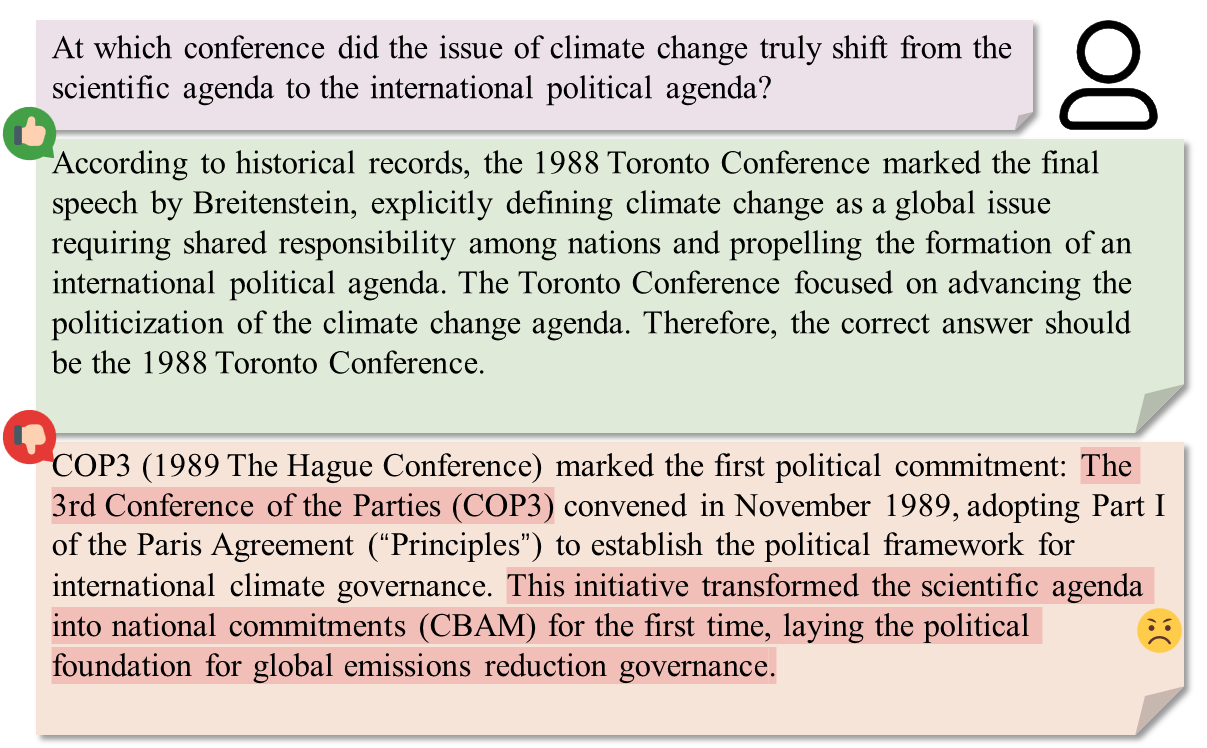
\includegraphics[width=\linewidth]{Images/Pang1.png}
\caption{Empirical evidence of hallucination phenomena in energy-carbon domain question answering. Comparative analysis reveals significant performance gaps between generic LLMs and domain-adapted models, with baseline models exhibiting critical errors such as incorrect emission factor application, confusion between Scope 1 and Scope 2 emissions, and misalignment with regulatory standards. These systematic observations demonstrate the critical necessity of domain-specific adaptation for reliable energy-carbon applications.}
\label{fig:overview}
\end{figure}

This work makes several key contributions. First, we empirically identify a long-context saturation regime in domain adaptation, showing that performance peaks at 6,000 samples (36M tokens) before declining due to attention dilution—a critical finding for compliance-heavy document processing. Second, we develop a hybrid system combining domain-adapted LLMs with retrieval-augmented generation, demonstrating that open models can rival commercial systems in specialized domains. Third, our comprehensive evaluation shows EC-LLM+RAG achieves 96.18\% factual accuracy and 36.18 BLEU-4, representing substantial improvements over baselines and establishing practical value for energy-carbon decision support.



\section{Related Work}\label{sec2}

\subsection{Domain-Specific Large Language Models}

Domain-specific adaptation of large language models has emerged as a powerful approach across high-stakes fields where specialized knowledge and precision are paramount. These models demonstrate that careful corpus curation and targeted fine-tuning can significantly enhance performance in domains requiring deep expertise.

In finance, BloombergGPT exemplifies this success, trained on 363 billion tokens of financial and general data to achieve state-of-the-art results~\cite{wu2023bloomberggpt}. Clinical adaptations show similar promise, with Med-PaLM achieving expert-level performance on medical examinations through instruction tuning~\cite{singhal2023large}. Legal domains benefit from models like LawLLM and LexGPT, which excel in case retrieval and judgment prediction by leveraging specialized legal corpora~\cite{shu2024lawllm,lee2023lexgpt}. These examples collectively demonstrate that domain-specific fine-tuning yields substantial improvements over general-purpose models.

Despite these advances in other verticals, the energy-carbon sector remains comparatively underserved in specialized LLM development.

\subsection{Fine-Tuning Strategies for Domain Adaptation}

Adapting general-purpose LLMs to specialized domains requires strategic fine-tuning approaches that balance domain expertise acquisition with computational efficiency. Key strategies include continued pretraining on domain corpora to align token distributions and semantic understanding, supervised instruction tuning (SFT) to teach domain-specific task formats and reasoning patterns, parameter-efficient fine-tuning (PEFT) techniques like LoRA to reduce computational requirements, and knowledge distillation from stronger teacher models.

In our work, we employ SFT on the energy-carbon instruction dataset, apply LoRA for efficient adaptation, and incorporate optional teacher-student distillation from DeepSeekR1-671B. Systematic ablation studies on dataset scale inform the optimal balance between performance gains and computational cost.

\subsection{Energy Systems AI and LLM Applications}

The energy sector has seen substantial AI adoption, particularly for operational tasks involving structured data. Comprehensive frameworks for home energy management systems~\cite{mahapatra2022hems}, reviews of photovoltaic maximum power point tracking~\cite{sarvi2022mppt_review}, and machine learning applications for district heating and cooling~\cite{ntakolia2022district_heating_ml_review} demonstrate the field's maturity in numerical optimization. Grid operations benefit from specialized models like LFLLM for load forecasting~\cite{liu2024lfllm}.

Recent efforts extend AI to more complex energy challenges. ElecBench provides a comprehensive 24-metric benchmark for power dispatch evaluation, while GAIA represents a dispatch-oriented LLM that surpasses LLaMA2 on ElecBench tasks~\cite{zhou2024elecbench,cheng2024gaia}. EnergyGPT addresses domain knowledge gaps through supervised fine-tuning of LLaMA 3.1-8B~\cite{chebbi2025energygptlargelanguagemodel}. A Joule commentary outlines future directions including data pipeline development, power system tool integration, and retrieval-augmented generation for safety-critical applications~\cite{majumder2024joule-llm-energy}.

As AI systems themselves contribute to carbon emissions, sustainable deployment becomes increasingly important. Frameworks like OpenCarbonEval and LLMCarbon provide quantitative tools for estimating the end-to-end carbon footprint of large AI models, covering both operational and embodied emissions~\cite{yu2024opencarboneval,faiz2023llmcarbon}. These developments inform efficient adaptation strategies and motivate the use of parameter-efficient techniques like LoRA in domain-specific LLM development.

\paragraph{Positioning of EC-LLM.} EC-LLM complements existing energy AI work by focusing on the policy and regulatory dimensions that underpin engineering decisions. While benchmarks like ElecBench and models like GAIA excel in operational tasks, EC-LLM addresses the critical need for reliable interpretation of unstructured policy documents and standards, bridging the gap between regulatory requirements and engineering implementation in the global energy transition.

\subsection{Energy-Carbon Domain Challenges and Initial Approaches}

While AI applications flourish in energy systems, the energy-carbon domain presents unique challenges requiring both engineering expertise and regulatory compliance. Initial attempts to adapt LLMs, such as RE-LLaMA~\cite{hemied2024re}, demonstrate feasibility but remain limited to narrow subdomains like hydrogen deployment and solar photovoltaic policies, lacking comprehensive coverage of integrated energy systems, carbon markets, and international carbon policies.

Recent studies explore AI applications in energy-carbon contexts. Machine learning models assess renewable energy integration effects and policy effectiveness for carbon emission reduction~\cite{jiang2023solution,spinti2023atikokan}. Carbon reduction strategies leverage AI for emission pathway generation and economic impact evaluation of carbon pricing mechanisms~\cite{wang2024ecological}.

However, existing models typically focus on specific subdomains, leaving a critical gap for integrated LLM capabilities that can handle the full spectrum of energy-carbon tasks—from policy evaluation and carbon market forecasting to emission reduction strategy development.



\section{Methodology}\label{sec3}

\subsection{Training Objectives and Process}
Our goal is to give a general large language model energy-carbon knowledge through supervised fine-tuning on carefully created instruction data. This can be seen as optimizing parameters under domain-specific constraints. The domain corpus consists of documents \(\mathcal{D} = \{ d_k \}_{k=1}^K\). From these, we create an instruction dataset of triples
\[\mathcal{S} = \{ (q_i, c_i, a_i) \}_{i=1}^N,\]
where \(q_i\) is a domain question, \(c_i\) is the related context (a policy excerpt, standard section, or report piece) from \(\mathcal{D}\) to support the answer, and \(a_i\) is the correct answer. Using a pretrained decoder model \(f_\theta\), inputs become token sequences \(x_i = [\mathrm{BOS};\, c_i;\, q_i]\), with targets \(y_i = a_i\).

The learning objective is to minimize the negative log-likelihood of targets given inputs (teacher-forced next-token prediction). This represents "learning domain knowledge through instructions": the model learns to follow grounded prompts and produce accurate, complete answers. In energy compliance situations, this means reducing domain-specific prediction errors while following regulatory and terminology rules, which supports decision-making needs. The mathematical details of the SFT objective are in Appendix~\ref{secA2}.

Using the dataset \(\mathcal{S}\), we train the model \(f_\theta\) with the SFT objective. Loss is calculated at the token level across answers and averaged over mini-batches. During training, we combine context and question as input sequences and use teacher-forcing for targets. For efficient adaptation, we apply Low-Rank Adapters (LoRA) to attention and feed-forward projections. For a weight matrix \(W\) in the frozen base model, we create trainable low-rank updates. We optimize these updates under the SFT objective while keeping base weights fixed, preserving general language ability while focusing on domain knowledge. The LoRA formulation details are in Appendix~\ref{secA2}.

Some experiments combine SFT with teacher distillation from stronger models to improve training stability and answer accuracy. Let \(p_T(\cdot\mid x)\) be the teacher distribution and \(p_{\theta}(\cdot\mid x)\) the student distribution. We add KL divergence minimization between them as an extra loss term. We don't use DPO/PPO in this work; our domain adaptation relies on SFT (with LoRA) and optional distillation. Distillation details are in Appendix~\ref{secA2}. The EC-LLM dataset is split into training/validation/test sets with an 80/10/10 ratio, stratified across the eight subfields in Table~\ref{tab:fullwidth}. We use AdamW optimizer with gradient accumulation to fit GPU memory and ensure stable training. Key settings are shown in Table~\ref{tab:train_params}.

\subsection{Dataset}

Building the EC-LLM dataset is a key part of this work, providing domain-specific knowledge for training language models in energy-carbon fields. As shown in Table~\ref{tab:fullwidth}, the dataset covers eight subfields divided into ten practical areas, such as policy analysis, carbon emission calculations, and energy efficiency assessments. This wide coverage ensures the dataset can support many different tasks in the energy-carbon domain.

\subsubsection{Data Sources}

The dataset was built using reliable, domain-relevant data from many different sources. File categories and distribution are shown in Table~\ref{tab:file_stats}. We focused on both credibility and variety. The sources include academic literature—peer-reviewed journals and conference papers on energy technologies, emission modeling, and sustainability (for example, Applied Energy and Renewable and Sustainable Energy Reviews); government laws and regulations—official documents on national energy management and carbon control, collected from government websites and legal databases; national and local policies—policy documents outlining national energy strategies, carbon neutrality goals, and region-specific guidelines; industry standards—national and international standards for energy efficiency, renewable energy technologies, and carbon emission monitoring, from organizations like ISO, IEC, and local regulatory bodies; company case studies—from major energy companies, showing real-world energy management and carbon reduction practices; and research reports—industry analysis, market trends, and reports from government and non-government organizations focused on carbon emissions and energy transition.

These sources were carefully selected for their relevance, accuracy, and comprehensiveness, creating a strong and diverse knowledge base for the energy-carbon sector.

\begin{table}[htbp]
\tbl{Dataset composition analysis revealing the distribution of energy-carbon policy documents. This analysis quantifies the corpus diversity across document types, providing the empirical foundation for training data curation and enabling informed decisions about domain coverage and knowledge representation.}{%
\begin{tabular*}{\linewidth}{@{\extracolsep{\fill}} l r r @{} }
    \toprule
    \textbf{Category} & \textbf{Files }& \textbf{Proportion (\%)} \\
    \midrule
    Dual Carbon Solutions & 36415 & 23.46 \\
    Hydrogen Energy Storage & 28949 & 18.65 \\
    Green Development & 28825 & 18.57 \\
    Carbon Accounting & 21143 & 13.62 \\
    Industry Research Reports & 15120 & 9.74 \\
    CCER & 11466 & 7.39 \\
    ESG Framework & 11137 & 7.18 \\
    Dual Carbon Tools & 1447 & 0.93 \\
    Dual Carbon Policies & 523 & 0.34 \\
    Carbon Inclusive & 190 & 0.12 \\
    \bottomrule
    \end{tabular*}}
\label{tab:file_stats}
\end{table}

\begin{table}[htbp]
\tbl{Question taxonomy analysis for energy-carbon domain knowledge assessment. This classification framework systematically categorizes query types to evaluate model performance across different cognitive levels, enabling targeted improvements in domain-specific question answering capabilities.}{%
    \begin{tabularx}{\linewidth}{@{} Y Y r Y Y r @{} }
    \toprule
    \textbf{Primary Category} & \textbf{Secondary Category} & \textbf{Total} & \textbf{Primary Category} & \textbf{Secondary Category} & \textbf{Total} \\
    \midrule
    {CCER}& Measurement and Inspection & 12485 & {Carbon Inclusion}& Carbon Inclusion Policies & 472 \\
     & Standards and Regulations & 4673 & & Carbon Inclusion Methodologies & 130 \\
     & Project Cases & 1563 & & Carbon Inclusion Research Reports & 29 \\
     & Strategy and System & 733 & {Dual Carbon Solutions}& Dual Carbon Standards & 234 \\
    {ESG System}& Standards and Ratings & 6108 & & Energy Synergy & 76 \\
     & ESG-related Papers & 4023 & & Research Reports & 14 \\
     & Cases and Research Reports & 1892 & & Near-Zero Carbon Areas & 13 \\
     & Corporate White Papers and Guidelines & 1879 & & Energy Optimization & 7 \\
     & Listed Company Reports & 61 & {Dual Carbon Policies}& National Policies & 21 \\
    {General Technology}& Implementation Methods & 5948 & & Local Policies & 1 \\
     & Technical Standards & 590 & {Green Development}& Renewable Energy & 28 \\
     & Monitoring and Verification & 205 & & Green Finance & 23 \\
     & Policies and Regulations & 1 & & Green Buildings & 22 \\
    {Dual Carbon Tools}& Trading and Finance & 19 & Hydrogen and Energy Storage & Hydrogen and Energy Storage & 13 \\
     & Market Data and Analysis & 3 & Others & Uncategorized & 5075 \\
     & Tool Templates and Manuals & 1 & Industry Research Reports & Industry Research Reports & 78 \\
    \bottomrule
    \end{tabularx}}
\label{tab:fullwidth}
\end{table}

\subsubsection{Data Processing and Quality Control}

To ensure the integrity and quality of the dataset, we employed a rigorous data processing and quality control pipeline. Text data was parsed using a multimodal large language model (MLLM)-based framework, capable of processing complex documents containing both textual and visual elements. The data cleaning process involved standardizing documents to ensure consistent machine-readable formats across various file types (e.g., PDF) and unifying character encodings. Automated algorithms, combined with manual verification, were used to filter out low-quality content and eliminate redundant or irrelevant information. Through multiple screening steps and random checks by domain experts, we ensured the accuracy, clarity, and domain relevance of the data, providing a solid foundation for subsequent model training.

\subsubsection{ Dataset Generation}
In the field of natural language processing, fine-tuning large language models (LLMs) for specific domains, such as energy-carbon knowledge, is crucial for achieving high performance. However, directly using general-domain datasets often fails to provide the depth and specificity required for specialized applications. To address this limitation, we propose a framework that combines self-instruction methods with retrieval-enhanced techniques to generate high-quality, domain-specific datasets for energy-carbon tasks, as shown in Fig.~\ref{fig:framework}.

Self-instruction methods reduce the reliance on manually annotated data by enabling LLMs to autonomously generate instruction data, such as questions and answers~\cite{wang2022self}. While effective for general tasks, these methods can struggle with specialized domains like energy-carbon knowledge, where generated responses may have high error rates. To address this, we combine retrieval-enhanced techniques to ensure generated questions are not only relevant but grounded in domain-specific corpora. Our dataset generation framework consists of three main stages: data collection and preprocessing, question generation, and context pairing.

For data collection and preprocessing, we gathered a diverse set of energy-carbon-related documents—academic papers, industry reports, and policy documents—creating the foundational corpus. The data underwent thorough preprocessing, including document normalization, content parsing, and data cleaning to ensure consistency and domain alignment.

In question generation, we use a dual-method strategy. First, content-based generation leverages a teacher LLM with Chain-of-Thought (CoT) prompting to guide the model through reasoning steps, extracting contextual segments and identifying key themes. This process generates 3-5 domain-specific questions for each document, which are then evaluated for length, syntactic correctness, and relevance. Second, vocabulary-based generation extracts keywords from the corpus and generates questions using predefined templates. Keywords are extracted from expert-curated lists, such as the IPCC Vocabulary Database, and filtered for quality to ensure alignment with domain-specific concepts, as shown in Table~\ref{tab:term_templates}.

Finally, the questions undergo filtering and deduplication. Low-quality questions are discarded, and duplicates are removed using MD5 hashing. This results in a high-quality, diverse, and non-redundant question pool ready for the next stage of model training.

\subsubsection{Knowledge Management Subsystem (RAG)}
To support dynamic policy environments, we introduce a knowledge management subsystem based on retrieval-augmented generation. During training, we use static context pairing to ground questions in their source documents and reduce computational overhead. At inference, the subsystem queries a curated, up-to-date store of policies, standards, and reports to supply relevant context, ensuring answers reflect the latest regulatory guidance. This bridges unstructured text and engineering decisions, improving reliability for decision support.

Formally, let \(g_{\mathrm{content}}(d)\) produce questions from document \(d\), and \(g_{\mathrm{template}}(v)\) produce template-based questions from term \(v\). Let \(\mathcal{Q} = \bigcup_{d\in\mathcal{D}} g_{\mathrm{content}}(d)\;\cup\;\bigcup_{v\in\mathcal{V}} g_{\mathrm{template}}(v)\) be all candidate questions, with \(\mathcal{V}\) the curated vocabulary. A deterministic pairing function \(m: \mathcal{Q} \to \mathcal{D}\) maps each question to its grounding context \(c=m(q)\). The instruction dataset becomes
\[\mathcal{S} = \big\{ \big(q,\, m(q),\, a\big) : q\in \mathcal{Q},\; a \text{ passes quality filters} \big\}.\]
This makes the data construction explicit as a mapping from corpus and vocabulary to grounded QA triples. Static pairing is used to build training examples; at inference time, retrieval can optionally be used to supply \(c\) if needed, but our learning objective remains the supervised loss in Eq.~\eqref{eq:sft}.



            \begin{table}[htbp]
            \centering
            \caption{Template-based question generation methodology for scalable knowledge extraction. This approach demonstrates how structured templates enable systematic generation of domain-specific questions, providing a reproducible method for creating large-scale training datasets while ensuring semantic diversity and knowledge coverage. The template column shows placeholders that are instantiated with specific domain entities in the generated questions.}
            \label{tab:term_templates}
            
            \begin{tabularx}{\linewidth}{@{} >{\raggedright\arraybackslash}p{0.18\linewidth} >{\raggedright\arraybackslash}X >{\raggedright\arraybackslash}X @{} }
            \toprule
            \textbf{Term} & \textbf{Template} & \textbf{Generated Question} \\
            \midrule
            Additionality & Given the context of \btexttt{[Policy X]}, how should a company in \btexttt{[Industry Y]} calculate its baseline under condition \btexttt{[Z]}? & Given the context of the CCER methodology, how should a manufacturing company in the steel industry calculate its baseline emissions under the condition of capacity expansion? \\
            Scope 1 Emissions & Under \btexttt{[Standard X]}, what are the compliance requirements for \btexttt{[Entity Y]} when reporting \btexttt{[Activity Z]}? & Under the GHG Protocol, what are the compliance requirements for a power plant when reporting direct combustion emissions? \\
            MRV Framework & Based on \btexttt{[Regulation X]} and considering \btexttt{[Context Y]}, what steps must be taken to ensure \btexttt{[Outcome Z]}? & Based on the national carbon market regulations and considering a renewable energy project, what steps must be taken to ensure accurate monitoring, reporting, and verification of emission reductions? \\
            \bottomrule
            \end{tabularx}
            \end{table}
            

 


\begin{figure*}[t]
\centering
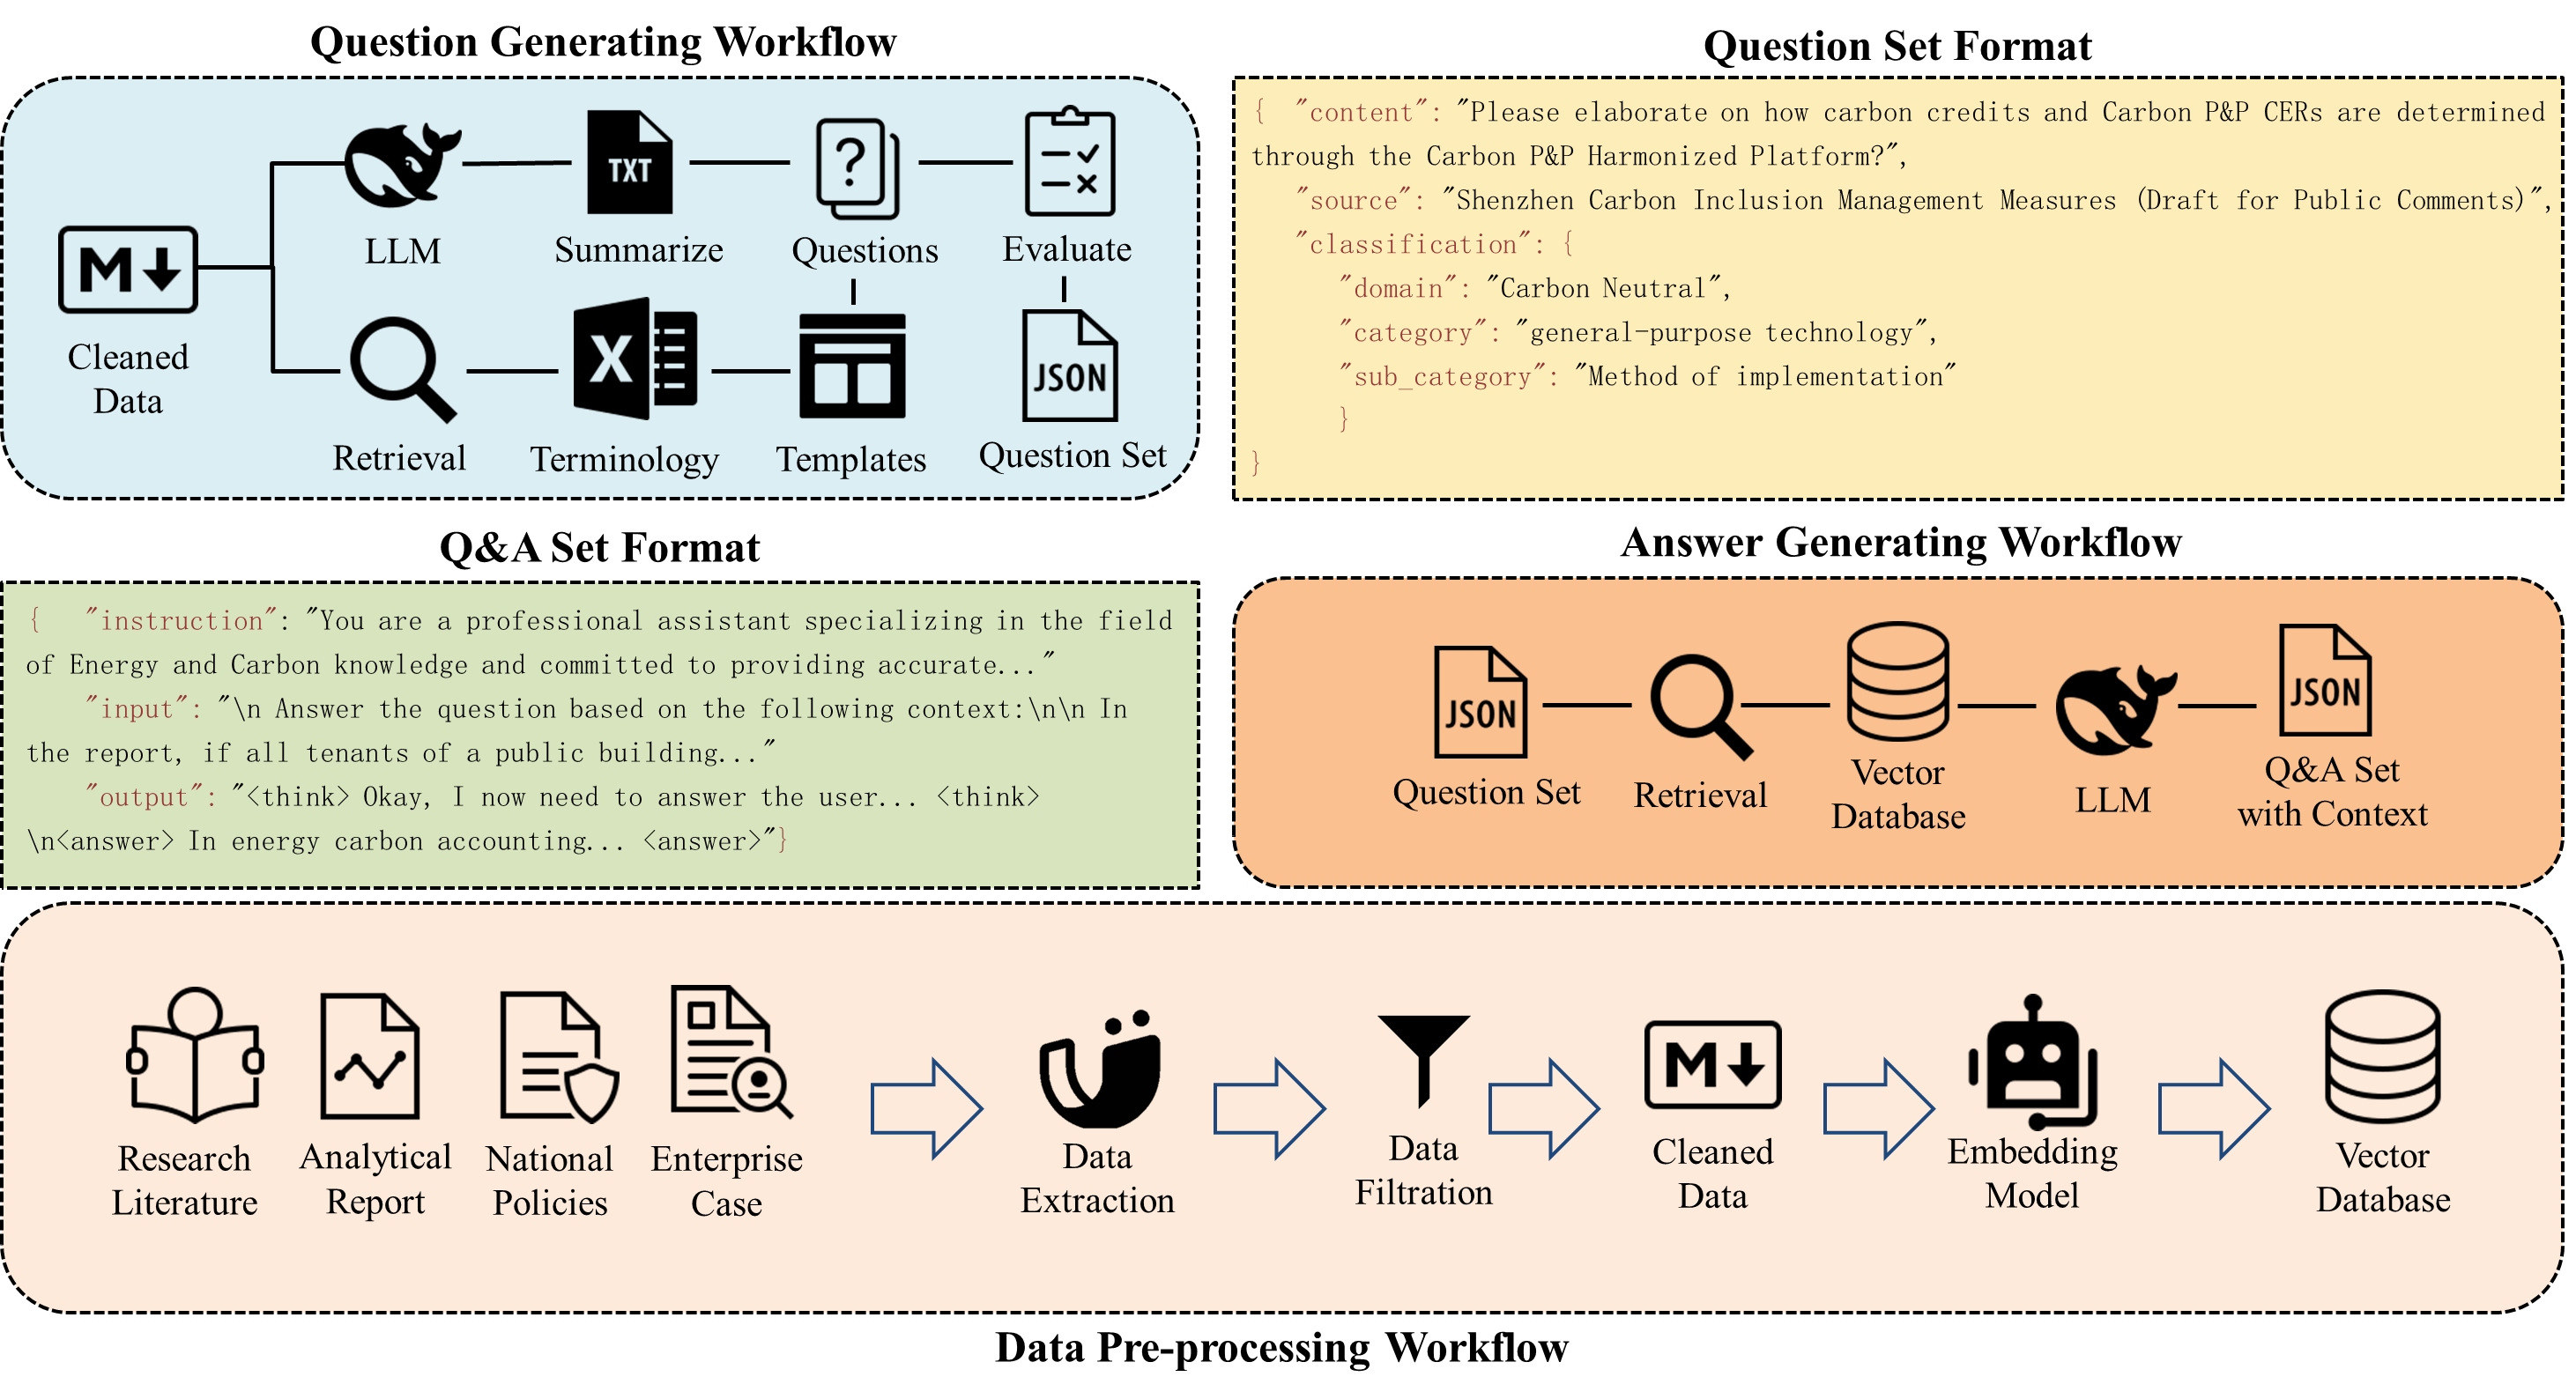
\includegraphics[width=\textwidth]{Images/Pang2.png}
\caption{Systematic data-curation pipeline for energy-carbon QA research. The process begins with the collection of diverse documents, including policy texts, technical standards, and academic literature. Through a rigorous pre-processing stage, these documents are normalized and segmented. The core of the pipeline involves a dual-strategy question generation phase: rule-based templates ensure coverage of key terminology, while generative models produce complex reasoning queries. Finally, answers are distilled from both retrieval-based and parametric sources, undergoing strict quality filtering. This pipeline is directly aligned with practical energy applications, ensuring that the resulting model can effectively support tasks such as automated carbon inventory verification and policy compliance checks.}
\label{fig:framework}
\end{figure*}

\subsection{Model}
The model architecture plays a key role in enabling the EC-LLM to perform well across diverse tasks in the energy-carbon sector. The architecture is designed to capture both domain-specific knowledge and broad general knowledge, ensuring strong performance in practical applications.

\subsubsection{Foundational Model Selection}
To meet the demands of dialogue applications in the energy-carbon sectors, EC-LLM adopts DeepSeek-Distill-Qwen-7B as its foundational model. This model is based on the Transformer decoder architecture and shares architectural characteristics with Qwen2.5, which is initialized from Qwen2.5-7B and fine-tuned using knowledge distillation from DeepSeek-R1. The original Qwen2.5-7B model was pre-trained on an extensive multilingual corpus comprising approximately 18 trillion tokens across 29 languages, including both Chinese and English. This large-scale, multilingual pretraining endows the model with broad general knowledge, multilingual capabilities, and strong reasoning abilities.

The distillation process further enhances the model's performance by incorporating high-quality reasoning datasets generated by DeepSeek-R1, with a focus on tasks such as mathematical problem-solving, programming, and logical reasoning. The resulting model, DeepSeek-Distill-Qwen-7B, supports a context window of 32,768 tokens, significantly exceeding many comparable models and enabling efficient handling of long-form inputs\textemdash{} an essential capability for domain-specific dialogue tasks that require long-context understanding~\cite{yang2025qwen3technicalreport}.

\subsubsection{Key Architectural Features}
The detailed architectural features of EC-LLM, including the Transformer Decoder structure, Grouped Query Attention (GQA), SwiGLU Activation Function, Attention QKV Biases, Rotary Positional Encoding (RoPE), and RMSNorm, are provided in Appendix \ref{secA1}. These features collectively contribute to the model's efficiency and performance in handling domain-specific tasks.

% Training Process merged into unified subsection above

\subsubsection{Training Setup and Parameters}
We split the EC-LLM dataset into training, validation, and test sets with an 80/10/10 ratio, stratified across the eight subfields listed in Table~\ref{tab:fullwidth}. Training uses AdamW with gradient accumulation to fit GPU memory while maintaining stable updates. Key configurations are summarized in Table~\ref{tab:train_params}.

\begin{table}[htbp]
\tbl{Systematic hyperparameter optimization framework for domain-specific model fine-tuning. This configuration presents the empirical design decisions that maximize model performance in the energy-carbon domain, providing a reproducible training protocol that balances computational efficiency with domain adaptation effectiveness.}{%
\small\setlength{\tabcolsep}{6pt}\renewcommand{\arraystretch}{1.1}
\begin{tabularx}{\linewidth}{@{} l l >{\raggedright\arraybackslash}X @{} }
\toprule
Parameter & Value & Rationale \\
\midrule
Base model & DeepSeek-Distill-Qwen-7B & Strong reasoning with moderate size \\
Context length & 8192 tokens (training) & Model supports 32,768; 8192 used for training efficiency \\
Batch size & 64 (via gradient accumulation) & Fits memory; stable updates \\
Learning rate & 2e-5 (AdamW) & Common for SFT; avoids overfitting \\
Optimizer & AdamW & Decoupled weight decay; stable convergence \\
LoRA rank & 16 (Q,K,V,O) & Parameter-efficient tuning \\
Epochs & 3 & Balance quality and compute \\
Teacher model & DeepSeekR1-671B & Distillation for domain alignment \\
\bottomrule
\end{tabularx}}
\label{tab:train_params}
\end{table}

\section{Results}\label{sec4}

\subsection{Baseline Model}
To evaluate EC-LLM, we compared it with several open-source baseline models and commercial state-of-the-art systems:

DeepSeek-R1-Distill-Qwen: Available in both 7B and 1.5B parameter versions, this model is fine-tuned with 800k high-quality inference samples from DeepSeek-R1. The 7B version excels in mathematical and logical reasoning, achieving impressive results on benchmarks like AIME 2024 (55.5\% pass rate) and MATH-500 (92.8\% pass rate), making it suitable for resource-constrained environments and carbon knowledge tasks. The 1.5B version, despite its smaller size, outperforms larger models like GPT-4o and Claude-3.5-Sonnet on similar tasks (83.9\% pass rate on MATH-500). Both models are open-source under Apache 2.0 and are highly efficient for energy-carbon knowledge applications, though the 1.5B model lacks coding and multilingual capabilities.

DeepSeek-R1-Distill-Llama-8B. Built on the Llama3.1-8B-Base foundation, this model achieves an 89.1\% pass rate on MATH-500 and performs well on tasks like GPQA Diamond (49.0\%). While strong in energy-carbon reasoning, it struggles with coding tasks, scoring poorly on LiveCodeBench and CodeForces. It follows the Llama3.1 open-source license.

GPT-4o. As a commercial state-of-the-art general-purpose model, GPT-4o serves as a strong baseline to demonstrate the value of domain-specific adaptation. We evaluated GPT-4o on a subset of 100 representative ECQA test samples to compare against EC-LLM's domain expertise. It is important to note that this comparison has limitations: GPT-4o was evaluated without access to our private energy-carbon knowledge base or domain-specific prompt engineering, and full-scale evaluation was constrained by API costs and rate limits. Our conclusion emphasizes that domain-adapted open models can rival commercial generalist models under domain constraints, rather than claiming universal superiority.

\subsection{Dataset Evaluation}
In constructing the High-Density Domain Instruction Dataset for energy-carbon knowledge, we evaluated the impact of data scale on model performance by partitioning the dataset into intervals ranging from 1,000 to 7,000 samples. The dataset's high-density nature stems from the long-context documents: with an average context length exceeding 6,000 tokens per sample, our 6,000-sample training set encompasses over 36 million tokens. To provide perspective, this token volume is roughly comparable to datasets with approximately 60,000 short-context samples (assuming 600 tokens per sample) from a token-normalized perspective, highlighting the importance of token-normalized rather than sample-count-based evaluation. To efficiently explore the dataset scaling laws, we initially used the DeepSeek-R1-Distill-Qwen-1.5B model for supervised fine-tuning (SFT) as a proxy, which allowed rapid iteration across multiple data scales. The final EC-LLM model, however, is trained on DeepSeek-Distill-Qwen-7B using the optimal 6,000-sample configuration identified through this scaling analysis. We assessed model performance across both objective and subjective dimensions. Objective metrics included BLEU-4~\cite{papineni2002bleu} and ROUGE (ROUGE-1, ROUGE-2, ROUGE-L)~\cite{lin2004rouge}, while subjective quality was evaluated using a Qwen2.5-14B model judge for semantic completeness, factual accuracy, and answer similarity. Specific results are shown in Table~\ref{tab:final_comprehensive_eval_en}. Examples of correct and incorrect answers as subjectively assessed by LLM are also provided in Table~\ref{tab:answer_comparison_revised}.

\begin{sloppypar}
\raggedright
Results demonstrated the efficacy of LoRA fine-tuning~\cite{hu2022lora}, with significant performance gains starting from 1,000 samples. As the dataset increased, performance continued to improve, with the training convergence loss decreasing from 1.80 to 1.45 and evaluation metrics steadily rising. A clear performance peak was observed at 6,000 samples, where BLEU (31.32), ROUGE-1 (56.21), ROUGE-2 (26.38), and ROUGE-L (30.83) reached their optimal values, indicating an ideal balance of knowledge volume and complexity.

However, when the dataset size was increased to 7,000 samples, performance declined sharply. Both training loss and evaluation scores worsened, with ROUGE-1 dropping from 56.21 to 53.13. This inflection point can be attributed to long-context noise and attention dilution: as the number of long-context samples increases beyond the optimal threshold, the model's attention mechanism struggles to maintain focus on critical information across extended sequences, leading to degraded performance. This phenomenon is particularly pronounced in domain-specific fine-tuning where policy documents and technical standards require precise attention to regulatory details. While the exact saturation point may vary across architectures and domains, our results indicate that long-context, compliance-heavy corpora exhibit an earlier saturation regime compared to short-context QA datasets. Based on these findings, the model trained on 6,000 samples with early stopping is optimal, achieving the highest evaluation scores and stable training dynamics, emphasizing the importance of data quality and density over sheer volume.
\end{sloppypar}


\begin{figure*}[t]
\centering
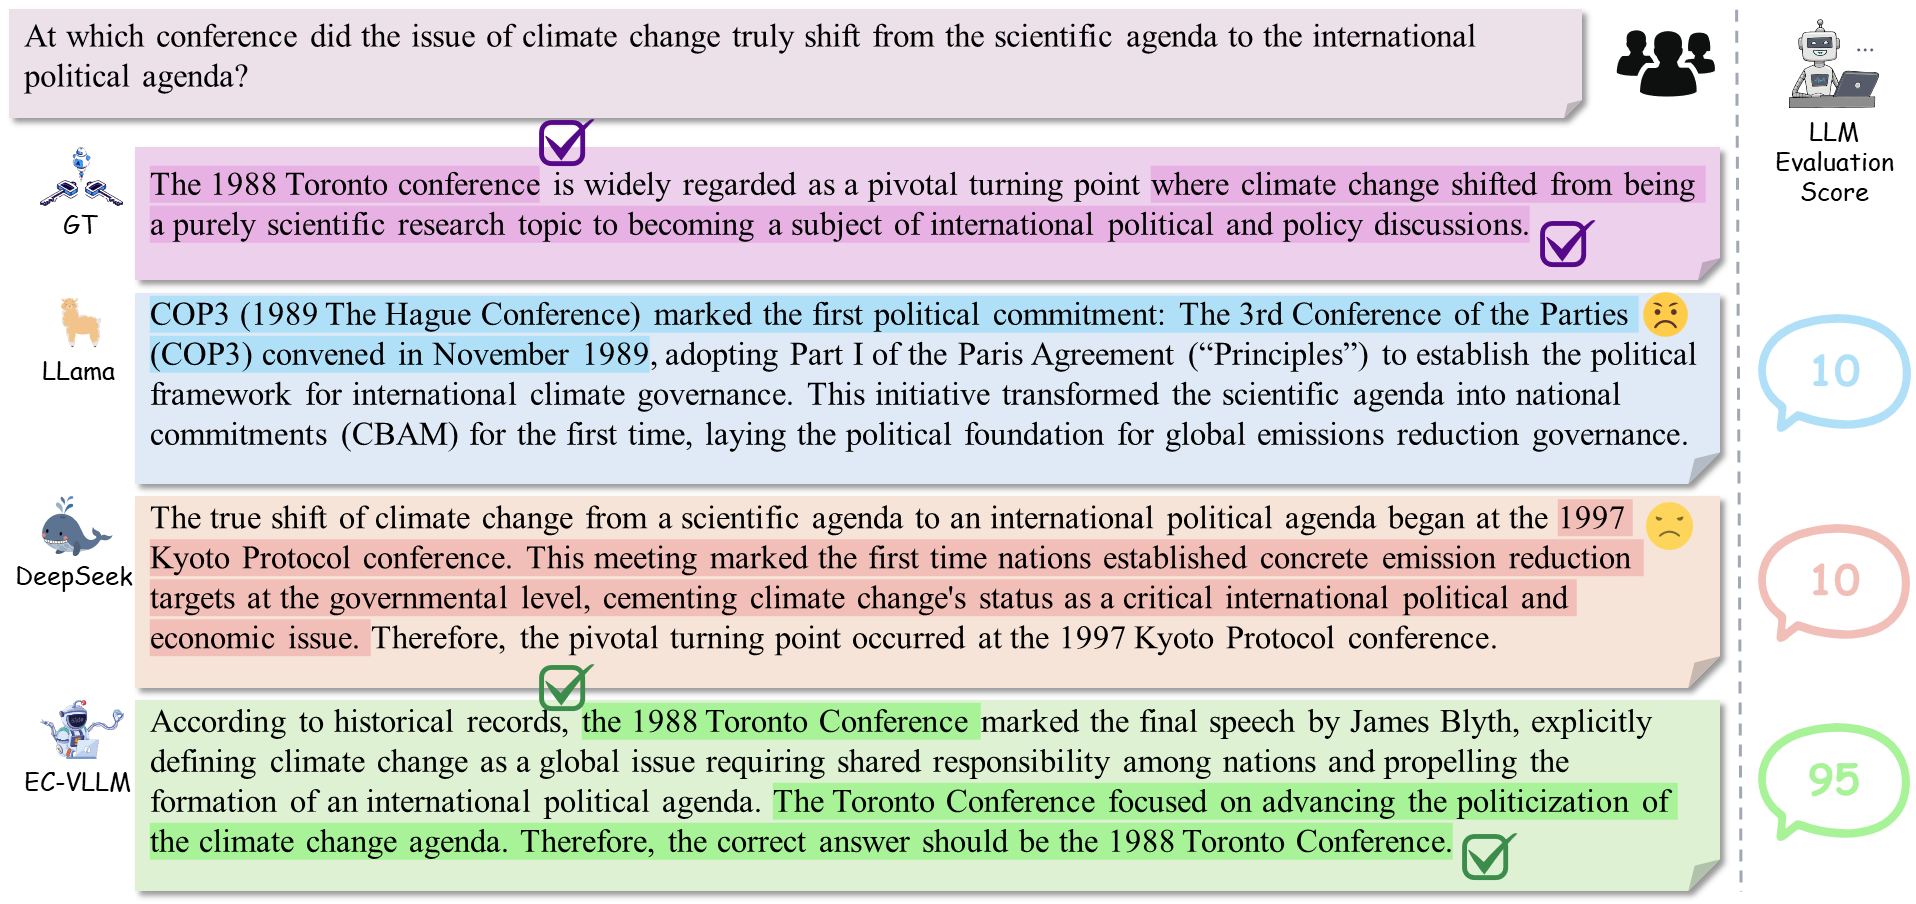
\includegraphics[width=\textwidth]{Images/Pang3.png}
\caption{Comparative analysis of hallucination phenomena across different training paradigms in energy-carbon question answering. Systematic evaluation reveals that baseline models generate factually incorrect responses and miss critical domain-specific details when handling specialized terminology and policy requirements. Our assessment framework employs semantic completeness analysis and factual accuracy validation to quantify answer quality, demonstrating that EC-LLM effectively suppresses hallucinations through domain-specific adaptation while maintaining comprehensive coverage of energy-carbon knowledge.}
\label{fig:results}
\end{figure*}

\begin{table}[htbp]
\tbl{Scaling law analysis revealing optimal training data size for domain-specific model performance. This systematic evaluation quantifies the relationship between dataset scale and model effectiveness, identifying the performance saturation point and providing evidence-based guidance for resource allocation in domain adaptation projects.}{%
\setlength{\tabcolsep}{1.8pt}\small\renewcommand{\arraystretch}{1.08}
\begin{tabular*}{\linewidth}{@{\extracolsep{\fill}} c c ccc ccc @{} }
\toprule
\textbf{Dataset Size} & \textbf{Train Loss} & \multicolumn{3}{c}{\textbf{Objective (Semantic)}} & \multicolumn{3}{c}{\textbf{Subjective (LLM)}} \\
\cmidrule(lr){3-5} \cmidrule(lr){6-8}
\textbf{(Rows)} & \textbf{(Approx.)} & \textbf{BLEU} & \textbf{ROUGE-1} & \textbf{ROUGE-L} & \textbf{Comp.} & \textbf{Acc.} & \textbf{Sim.} \\
\midrule
Base Model & N/A & 13.21 & 36.22 & 18.15 & 73.97 & 73.98 & 60.43 \\
1000 & $\sim$1.80 & 18.66 & 43.52 & 24.84 & 74.98& 77.22 & 61.12 \\
2000 & $\sim$1.50 & 26.01 & 50.86 & 27.56 & 81.94 & 85.48 & 70.47 \\
3000 & $\sim$1.67& 25.90 & 51.58 & 26.94 & 79.18 & 83.53 & 68.23 \\
4000 & $\sim$1.72 & 27.43 & 53.59 & 27.93 & 81.27 & 84.89 & 70.5 \\
5000 & $\sim$1.47 & 29.60 & 54.89 & 29.68 & 81.89 & 85.83 & 71.04 \\
\textbf{6000} & \textbf{$\sim$1.45} & \textbf{31.32} & \textbf{56.21} & \textbf{30.83} & \textbf{82.42} & \textbf{86.21} & \textbf{71.71} \\
7000 & $\sim$1.93 & 27.40 & 53.13 & 28.07 & 81.67 & 85.76 & 70.73 \\
\bottomrule
\end{tabular*}}
\label{tab:final_comprehensive_eval_en}
\end{table}

\begin{table}[htbp]
\tbl{Qualitative error analysis framework for validating model performance in domain-specific scenarios. This comparative assessment demonstrates how structured LLM-based evaluation identifies critical performance gaps, providing actionable insights for model improvement through detailed analysis of semantic completeness, factual accuracy, and answer similarity across different application domains.}{%
    \small\setlength{\tabcolsep}{3.5pt}\renewcommand{\arraystretch}{1.12}
    \begin{tabularx}{\linewidth}{@{} >{\raggedright\arraybackslash}p{.20\linewidth} >{\raggedright\arraybackslash}p{.24\linewidth} >{\raggedright\arraybackslash}p{.24\linewidth} >{\raggedright\arraybackslash}p{.26\linewidth} @{} }
    \toprule
    \textbf{Case Topic} & 
    \textbf{Correct Answer Example (Simplified)} & 
    \textbf{Incorrect Answer Example (Simplified)} & 
    \textbf{Scoring Analysis \& Feedback} \\
    \midrule
    
    % --- ROW 1: MANGROVE AUDIT ---
    \textbf{Case 1:} \newline Mangrove Ecosystem Monitoring Compliance Audit & 
    \textbf{Clear structure, comprehensive coverage} \newline
    Compliance plan review; data management; QC and standard implementation; validation \& verification; legal ownership; appendices \& normative documents. & 
    \textbf{Key points missing, logic not rigorous} \newline
    Incomplete compliance check; vague monitoring schedule; partial QC analysis; insufficient technical validation; fragmented reporting. & 
    \textbf{Scoring} (0--100): \newline
    Semantic completeness 90; factual accuracy 95; answer similarity 85. \newline
    \textbf{Feedback:} Include legal ownership and environmental/social impact to complete the audit description. \\
    \midrule
    
    % --- ROW 2: WATER SOFTENER ---
    \textbf{Case 2:} \newline Water Softener Monitoring Requirements & 
    \textbf{Precise focus, captures the core} \newline
    Effluent hardness and pH monitoring; smart alerts for consumables; standards per GB/T 5750; manufacturer documentation. & 
    \textbf{Confused content, misses the point} \newline
    Lists irrelevant emission indicators; lacks hardness/pH; repetitive and off-topic. & 
    \textbf{Scoring} (0--100): \newline
    Semantic completeness 20; factual accuracy 40; answer similarity 5. \newline
    \textbf{Feedback:} Focus on monitoring/maintenance functions and include hardness and pH monitoring. \\
    \midrule
    \multicolumn{4}{@{}p{\linewidth}@{}}{\textbf{Managerial Implications:} Improvements in factual accuracy and semantic completeness translate into shorter verification cycles and lower compliance risk for carbon auditors. In practice, EC-LLM reduces manual lookup of standards and consolidates policy interpretation, enabling faster decision support in energy systems operations.} \\
    \bottomrule
    \end{tabularx}}
\label{tab:answer_comparison_revised}
\end{table}



\subsection{Results and Analysis}
We evaluated the performance of three baseline models: Qwen2.5-1.5B, Qwen2.5-7B, and Llama3.1-8B, under different training paradigms: base models, base models with Distillation, base models with Supervised Fine-Tuning (SFT), and base models with both SFT and Distillation. Additionally, we evaluated EC-LLM (trained on DeepSeek-Distill-Qwen-7B with SFT and Distillation using the optimal 6,000-sample dataset identified in Section~\ref{sec4}) with and without the retrieval-augmented generation (RAG) subsystem to assess the contribution of the knowledge management component. The evaluation was conducted on an energy-carbon question answering (ECQA) test set. The assessment was based on objective lexical metrics (BLEU, ROUGE-1, ROUGE-2, ROUGE-L) and subjective quality (semantic completeness, factual accuracy, and answer similarity), with the latter assessed using the Qwen2.5-14B model. To validate the reliability of LLM-based evaluation, we conducted a human evaluation study with three domain experts (policy analysts and energy engineers) on a subset of 50 representative samples, achieving a Spearman correlation of 0.82 between human ratings and LLM-judged scores for factual accuracy, confirming the validity of our automated assessment protocol. In addition, we reference modern learned metrics such as COMET and BLEURT that better correlate with human judgments in many generation tasks~\cite{rei2020comet,sellam2020bleurt}. The detailed results are presented in Table~\ref{tab:ecqa_results}. Moreover, to demonstrate how EC-LLM successfully suppresses hallucinations through training, Fig.~\ref{fig:results} shows the outputs of different models addressing the same problem. 

% --- Table 7A: Objective metrics ---
\begin{table}[htbp]
\tbl{Quantitative performance benchmarking across different training paradigms using objective lexical metrics. This systematic comparison provides empirical evidence that the combination of supervised fine-tuning and knowledge distillation achieves optimal domain adaptation, establishing a performance baseline for energy-carbon question answering tasks. $^*$GPT-4o results are based on a representative subset of 100 samples without access to our private energy-carbon knowledge base, evaluated under API constraints.}{%
\setlength{\tabcolsep}{1.8pt}\footnotesize\renewcommand{\arraystretch}{1.06}
\begin{tabular*}{\linewidth}{@{\extracolsep{\fill}} l cccc @{} }
\toprule
\textbf{Models} & \textbf{BLEU} & \textbf{ROUGE-1} & \textbf{ROUGE-2} & \textbf{ROUGE-L} \\
\midrule
Qwen2.5-1.5B & 3.76 & 24.22 & 6.76 & 11.4 \\
Qwen2.5-7B & 10.53 & 33.36 & 10.84 & 18.23 \\
Llama3.1-8B & 19.07 & 48.53 & 17.73 & 21.52 \\
\midrule
Qwen2.5-1.5B+Distill & 13.21 & 36.22 & 13.11 & 18.15 \\
Qwen2.5-7B+Distill & 18.38 & 43.47 & 16.98 & 24.74 \\
Llama3.1-8B+Distill & 24.13 & 49.45 & 20.9 & 27.44 \\
\midrule
Qwen2.5-1.5B+SFT & 19.64 & 49.92 & 18.17 & 21.52 \\
Qwen2.5-7B+SFT & 21.24 & 50.87 & 19.61 & 22.77 \\
Llama3.1-8B+SFT & 28.14 & 59.02 & 25.01 & 26.11 \\
\midrule
Qwen2.5-1.5B+SFT+Distill & 31.32 & 56.21 & 26.38 & 30.83 \\
Qwen2.5-7B+SFT+Distill & 34.32 & 59.37 & 28.98 & 32.75 \\
GPT-4o$^*$ & 28.45 & 55.12 & 24.67 & 30.21 \\
\textbf{EC-LLM} & \textbf{35.62} & \textbf{60.14} & \textbf{29.48} & \textbf{33.3} \\
\textbf{EC-LLM+RAG} & \textbf{36.18} & \textbf{61.23} & \textbf{30.12} & \textbf{33.89} \\
\bottomrule
\end{tabular*}}
\label{tab:ecqa_results}
\end{table}

% --- Table 7B: Subjective metrics ---
\begin{table}[htbp]
\tbl{Subjective quality assessment validating model performance through LLM-based evaluation. This comprehensive analysis demonstrates that our domain adaptation approach significantly improves semantic completeness, factual accuracy, and answer similarity, providing robust evidence for the effectiveness of combined supervised fine-tuning and knowledge distillation in specialized domains. $^*$GPT-4o results are based on a representative subset of 100 samples without access to our private energy-carbon knowledge base, evaluated under API constraints.}{%
\setlength{\tabcolsep}{1.4pt}\footnotesize\renewcommand{\arraystretch}{1.05}
\begin{tabular*}{\linewidth}{@{\extracolsep{\fill}} >{\raggedright\arraybackslash}p{.35\linewidth} ccc ccc @{} }
\toprule
\textbf{Models} & \textbf{Sem-Pass} & \textbf{Fact-Pass} & \textbf{Sim-Pass} & \textbf{Sem-Avg} & \textbf{Fact-Avg} & \textbf{Sim-Avg} \\
\midrule
Qwen2.5-1.5B & 2.76\% & 11.16\% & 0.60\% & 36.64 & 48.69 & 32.25 \\
Qwen2.5-7B & 15.95\% & 29.56\% & 1.47\% & 56.53 & 62.9 & 45.38 \\
Llama3.1-8B & 84.75\% & 69.51\% & 5.12\% & 82.76 & 82.98 & 68.99 \\
\midrule
Qwen2.5-1.5B+Distill & 52.92\% & 47.08\% & 6.04\% & 73.97 & 73.98 & 60.43 \\
Qwen2.5-7B+Distill & 58.87\% & 53.69\% & 7.64\% & 65.17 & 70.1 & 57.57 \\
Llama3.1-8B+Distill & 90.96\% & 80.12\% & 6.02\% & 83.43 & 85.09 & 71.53 \\
\midrule
Qwen2.5-1.5B+SFT & 71.76\% & 66.03\% & 2.91\% & 80.66 & 80.75 & 66.35 \\
Qwen2.5-7B+SFT & 85.87\% & 71.74\% & 5.01\% & 82.98 & 83.22 & 69.3 \\
Llama3.1-8B+SFT & 89.99\% & 82.76\% & 8.70\% & 84.24 & 86.64 & 72.3 \\
\midrule
Qwen2.5-1.5B+SFT+Distill & 87.58\% & 78.92\% & 7.82\% & 82.42 & 86.21 & 71.71 \\
Qwen2.5-7B+SFT+Distill & 95.19\% & 89.58\% & \textbf{11.02}\% & 84.41 & 87.63 & 73.76 \\
GPT-4o$^*$ & 91.23\% & 88.50\% & 9.34\% & 83.67 & 87.12 & 72.45 \\
\textbf{EC-LLM} & \textbf{96.59}\% & \textbf{95.39}\% & 10.22\% & \textbf{84.92} & \textbf{88.84} & \textbf{74.95} \\
\textbf{EC-LLM+RAG} & \textbf{97.12}\% & \textbf{96.18}\% & \textbf{11.45}\% & \textbf{85.34} & \textbf{89.42} & \textbf{75.61} \\
\bottomrule
\end{tabular*}}
\label{tab:ecqa_results_b}
\end{table}


As illustrated in Tables~\ref{tab:ecqa_results} and \ref{tab:ecqa_results_b}, the combination of SFT and Distillation consistently yielded the best performance across all models and metrics. EC-LLM achieved the highest scores overall across BLEU and ROUGE metrics, and also excelled in LLM-judged semantic completeness and factual accuracy. Notably, on a representative subset of 100 samples where GPT-4o was evaluated without access to our private energy-carbon knowledge base, GPT-4o achieved a factual accuracy of 88.50\%, which EC-LLM+RAG surpasses (96.18\%). This comparison demonstrates that domain-adapted open models can rival commercial generalist models under domain constraints, though we acknowledge that GPT-4o's performance could potentially improve with domain-specific prompt engineering or access to specialized knowledge bases. The integration of the RAG subsystem (EC-LLM+RAG) further improved performance, particularly in factual accuracy (96.18\% vs. 95.39\%) and ROUGE-1 (61.23 vs. 60.14), demonstrating the value of retrieval-augmented generation for accessing up-to-date policy documents and technical standards. These results underscore that both SFT for domain adaptation, Distillation for knowledge transfer, and RAG for dynamic knowledge access are crucial for achieving state-of-the-art performance in the ECQA domain.

SFT significantly improved the models' lexical and structural alignment with domain-specific knowledge. Comparing "Base Models" with "Base Models + SFT"  we observe substantial gains across all metrics. For instance, the Llama3.1-8B model's factual accuracy (factual\_pass) improved from 69.51\% to 82.76\% after SFT. The Qwen2.5-1.5B+SFT model showed remarkable relative improvement, with BLEU increasing from 3.76 to 19.64 and ROUGE-2 from 6.76 to 18.17. This confirms that SFT effectively enhances models with domain-specific knowledge, especially for smaller models. 

Distillation, when applied to base models ("Base Models + Distill"), also contributed positively to performance. For example, Qwen2.5-1.5B+Distill showed a significant jump in BLEU from 3.76 to 13.21 and semantic\_pass from 2.76\% to 52.92\% compared to its base counterpart. This suggests that knowledge transfer from a larger or more expert model through distillation can effectively improve smaller models, making them more robust and accurate. 

The most pronounced improvements were observed when SFT and Distillation were combined ("Base Models + SFT + Distill"). This synergy highlights that these two techniques complement each other. SFT customizes the model to the target domain, while Distillation further refines its knowledge and efficiency, often leading to better generalization and performance. For example, Qwen2.5-7B+SFT+Distill achieved a factual\_pass of 89.58\%, a substantial increase over both Qwen2.5-7B+Distill (53.69\%) and Qwen2.5-7B+SFT (71.74\%). EC-LLM, built on DeepSeek-Distill-Qwen-7B with SFT and Distillation, achieved the highest factual\_pass of 95.39\%, demonstrating the combined power of these methods. 

While larger models like Llama3.1-8B consistently achieved high absolute scores, EC-LLM (based on DeepSeek-Distill-Qwen-7B) demonstrates that the combination of strong base model capabilities, domain-specific fine-tuning, and knowledge distillation can achieve state-of-the-art performance. The relative improvements after SFT or SFT+Distillation were sometimes more dramatic for smaller models, suggesting that larger pre-trained models already possess significant linguistic competence, and SFT primarily refines them for specific domains. Smaller models, in contrast, experience a "great leap" in competence, highlighting the transformative potential of these techniques for resource-efficient models, allowing them to closely rival larger models in domain-specific tasks. 

In summary, the combination of SFT and Distillation proves highly effective for adapting models to the energy-carbon domain, yielding substantial improvements in both objective and subjective metrics. EC-LLM, built on DeepSeek-Distill-Qwen-7B with SFT and Distillation, achieves peak performance in the energy-carbon domain, demonstrating that domain-specific adaptation can effectively leverage the model's strong reasoning capabilities and long-context understanding. Factual accuracy emerges as a key improvement, ensuring the reliability of the model's outputs. The model's 32,768-token context window enables effective handling of long policy documents and technical standards, making it well-suited for compliance-critical applications in the energy-carbon sector. 



\section{Limitations and Future Work}\label{sec5}

Despite promising results, EC-LLM has several limitations that pave the way for future improvements. First, the model currently operates as a knowledge layer, focusing on question answering and information retrieval tasks. While our experiments demonstrate strong performance on ECQA, direct integration with downstream decision support workflows (such as automated MRV systems or carbon market forecasting tools) remains future work. The current system provides reliable knowledge grounding, but full decision support requires integration with optimization algorithms, simulation engines, and specialized emissions databases. Second, the model currently relies on a static dataset, whereas the energy-carbon domain is highly dynamic. Future work should focus on developing a continual learning pipeline to keep the model up-to-date with real-time data, ensuring its long-term relevance. Additionally, while the model has multilingual potential, expanding its training to include more languages and evaluating its performance in cross-lingual tasks will enhance its global applicability.

Further, human-in-the-loop evaluations with domain experts, such as policy analysts and energy engineers, will be crucial for refining the model's accuracy and usability. To improve its trustworthiness, future versions should enhance interpretability and traceability to source documents. Lastly, integrating EC-LLM with external tools, like specialized emissions databases or carbon modeling systems, will elevate its functionality, enabling more complex problem-solving tasks. Nevertheless, ECQA captures the dominant knowledge bottleneck in current energy-carbon workflows, where practitioners spend substantial effort interpreting standards rather than executing numerical optimization. By addressing these areas, EC-LLM can evolve from a knowledge layer to a comprehensive decision support system, driving the transition to a sustainable, low-carbon future.




\relax

\section*{Declarations}

\begin{itemize}
\item \textbf{Funding}: No funding was received for conducting this study.
\item \textbf{Competing interests}: The authors declare that they have no competing interests.
\item \textbf{Data availability statement}: The processed instruction datasets (question-context-answer triples) generated and analyzed during the current study are available in the EC-LLM repository, \url{https://github.com/FAyyn/EC\_LLM}. Due to copyright constraints associated with government policy documents, industry standards, and proprietary reports, we release processed instruction data and document identifiers/metadata rather than raw PDFs. This approach ensures reproducibility while respecting intellectual property rights. The repository includes: (1) processed QA instruction pairs (derived data), (2) document identifiers linking to publicly accessible sources (e.g., ISO standards, government website URLs), and (3) metadata files containing source categories, processing timestamps, and quality control flags.
\item \textbf{Code availability}: The source code for the models and experiments is available at \url{https://github.com/FAyyn/EC\_LLM}.
\item \textbf{Author contributions}: NaiPeng Wang led the manuscript writing and conducted the main experimental work. Linjie Tong and Longtao Zhang provided assistance with experiments and data processing. Chengxin Pang and Xiaoguang Zhu provided guidance on theoretical framework and research direction.
\end{itemize} 




\appendix

\section{Detailed Architectural Features}\label{secA1}

We include these architectural details for completeness and reproducibility. EC-LLM does not claim novelty in core transformer components; instead, our contribution lies in how these established architectures are adapted and evaluated under compliance-critical, long-context energy-carbon settings. The following sections document the architectural choices that enable EC-LLM's strong performance in domain-specific tasks.

EC-LLM integrates a suite of advanced architectural features to improve performance and efficiency in natural language processing tasks:

\paragraph{Transformer Decoder Architecture} Utilizes self-attention to model long-range dependencies in sequential data, enabling sophisticated language understanding and generation.

\paragraph{Grouped Query Attention (GQA)} Reduces computational complexity by grouping query vectors while sharing key and value projections, allowing for faster inference without sacrificing accuracy.

\paragraph{SwiGLU Activation Function} In the feedforward neural network (FFN) layer, EC-LLM employs the Swish-Gated Linear Unit (SwiGLU) activation. Compared to traditional activation functions like ReLU, SwiGLU introduces a gating mechanism that enhances the model's capacity to represent complex patterns in data, thereby improving overall performance~\cite{shazeer2020glu}. The detailed mathematical formulation is provided in Appendix~\ref{secA2}.
To compare the activation effects of SwiGLU and ReLU, Yang et al. conducted comparative experiments based on the Qwen2.5-7B architecture, with results consolidated from ablation experiments. SwiGLU reduces confusion by 14.6\% compared to ReLU, primarily due to the dynamic filtering of information through the gating mechanism, which enhances nonlinear expression capabilities. SwiGLU increases the number of parameters by approximately 15\% due to the bilinear transformation, but this is compensated for by group query attention (GQA). In a 1M-token code understanding task, SwiGLU achieves a 9.2\% higher semantic recall rate than ReLU, as the smoothing of gradients mitigates the decay of long-range dependencies. As such, SwiGLU consistently outperforms ReLU and GELU in language modeling tasks, with particularly significant gains in low-resource tasks and long-context scenarios. Its computational overhead can be optimized through the Mixture-of-Experts (MoE) architecture or GQA, making the actual deployment cost manageable \cite{yang2025qwen2}.

\paragraph{Attention QKV Biases} Learnable biases are added to the Query, Key, and Value projections in the attention mechanism. These biases help stabilize training and improve model adaptability across diverse input types. Although specific implementation details remain undisclosed, QKV biases are considered beneficial for enhancing robustness.

\paragraph{Rotary Positional Encoding (RoPE)} To encode both relative and absolute positional information, EC-LLM employs RoPE, which applies rotational transformations to query and key vectors~\cite{su2024roformer}. By gradually increasing the RoPE base frequency to 10,000,000, the Qwen team solved the extrapolation bottleneck of long-sequence position encoding. Combined with the DCA mechanism, the model achieved an accuracy rate of 95.1\% in the 1M token Passkey Retrieval task, with a 3.2-6.7-fold improvement in memory efficiency~\cite{yang2025qwen2}. RoPE’s base frequency is adjusted based on model size, allowing for flexible generalization to inputs of varying lengths\textemdash{} particularly important for long-context scenarios.

\paragraph{RMSNorm for Normalization} EC-LLM adopts Root Mean Square Normalization (RMSNorm) in place of traditional LayerNorm. RMSNorm offers higher computational efficiency and enhanced training stability, especially in large-scale training settings~\cite{zhang2019root}. The detailed formulation is provided in Appendix~\ref{secA2}.

\paragraph{Activation Function Ablation} Under identical training settings on Qwen2.5-7B, SwiGLU achieved the best overall trade-off: BLEU-4 of 31.3 and factual accuracy of 86.2\%, while maintaining competitive inference speed (1480 tok/s) and acceptable GPU memory usage (10.8 GB). In comparison, GELU reached BLEU-4 of 27.6 and factual accuracy of 82.1\% (1420 tok/s; 10.1 GB), and ReLU reached BLEU-4 of 24.1 and factual accuracy of 78.3\% (1520 tok/s; 9.2 GB). These observations support the choice of SwiGLU in EC-LLM.

\section{Mathematical Formulations}\label{secA2}

\subsection{SFT Objective}
The learning objective is to minimize the negative log-likelihood of targets conditioned on inputs (teacher-forced next-token prediction):
\begin{equation}
\label{eq:sft}
\mathcal{L}_{\mathrm{SFT}}(\theta) 
= \sum_{i=1}^{N} \sum_{t=1}^{T_i} -\log p_{\theta}\big(y_i^{(t)} \mid y_i^{(<t)}, x_i\big).
\end{equation}

\subsection{LoRA Updates}
For a weight matrix \(W\) in the frozen base model, we parameterize a trainable low-rank update:
\begin{equation}
W \leftarrow W_0 + \Delta W,\quad \Delta W = A B,\quad A \in \mathbb{R}^{d\times r},\; B \in \mathbb{R}^{r\times d},\; r\ll d.
\end{equation}

\subsection{Distillation Loss}
We minimize the KL divergence between the teacher and student distributions:
\begin{equation}
\mathcal{L}_{\mathrm{Distill}}(\theta) = \sum_{i} \mathrm{KL}\big(p_T(\cdot\mid x_i)\,\big\|\, p_{\theta}(\cdot\mid x_i)\big),\quad \mathcal{L}(\theta) = \mathcal{L}_{\mathrm{SFT}}(\theta) + \lambda \, \mathcal{L}_{\mathrm{Distill}}(\theta),
\end{equation}
with \(\lambda\) a small positive coefficient.

\subsection{SwiGLU Activation}
The Swish-Gated Linear Unit (SwiGLU) activation is defined as:
\begin{equation}
    \text{SwiGLU}(x, y) = x \cdot \sigma(y),
\end{equation}
where $\sigma$ denotes the sigmoid function. Here, $x$ and $y$ denote the pre-activation linear outputs of two parallel feed-forward transformations.

\subsection{RMSNorm}
RMSNorm normalizes input vectors using their root mean square value:
\begin{equation}
    \text{RMSNorm}(x) = \frac{x}{\sqrt{\frac{1}{n} \sum_{i=1}^{n} x_i^2 + \epsilon}}
\end{equation}

\section{Evaluation Metrics Definitions}\label{secA3}

We employ a rigorous evaluation protocol involving both lexical and model-judged metrics to quantify performance. Let the test set be \(\mathcal{T}=\{(q_j,c_j,a_j)\}_{j=1}^{M}\). Given inputs \(x_j=[\mathrm{BOS};\,c_j;\,q_j]\), the model predicts \(\hat{a}_j=f_{\theta}(x_j)\).

\paragraph{Lexical metrics} We compute BLEU-4 and ROUGE to measure textual overlap. BLEU is defined as:
\begin{equation}
\mathrm{BLEU} = \mathrm{BP} \cdot \exp\Big(\sum_{n=1}^{4} w_n \log p_n\Big),\quad \mathrm{BP} = \begin{cases}
1 & \text{if } L_{\hat{a}} > L_a,\\
\exp\big(1 - \tfrac{L_a}{L_{\hat{a}}}\big) & \text{otherwise,}
\end{cases}
\end{equation}
where \(p_n\) is the modified n-gram precision, \(w_n\) are uniform weights, and \(L_a, L_{\hat{a}}\) denote reference and hypothesis lengths. For ROUGE-L, we use the longest common subsequence (LCS)-based F-score:
\begin{equation}
\mathrm{ROUGE\text{-}L} = \max_{\mathrm{LCS}} \; \mathrm{F}\text{-}\mathrm{score}(\mathrm{precision},\, \mathrm{recall}).
\end{equation}

\paragraph{LLM-judged metrics} To capture semantic correctness, we define three scalar scoring functions using an external judge model: semantic completeness \(S_{\mathrm{sem}}(x_j,\hat{a}_j)\), factual accuracy \(S_{\mathrm{fact}}(x_j,\hat{a}_j)\), and answer similarity \(S_{\mathrm{sim}}(x_j,\hat{a}_j)\), each normalized to \([0,100]\). With thresholds \(\tau_{\mathrm{sem}}, \tau_{\mathrm{fact}}, \tau_{\mathrm{sim}}\), the pass-rates are calculated as:
\begin{align}
\mathrm{Pass}_{\mathrm{sem}} &= \frac{1}{M}\sum_{j} \mathbf{1}\bigl\{S_{\mathrm{sem}}(x_j,\hat{a}_j)\ge \tau_{\mathrm{sem}}\bigr\},\\[2pt]
\mathrm{Pass}_{\mathrm{fact}} &= \frac{1}{M}\sum_{j} \mathbf{1}\bigl\{S_{\mathrm{fact}}(x_j,\hat{a}_j)\ge \tau_{\mathrm{fact}}\bigr\},\\[2pt]
\mathrm{Pass}_{\mathrm{sim}}  &= \frac{1}{M}\sum_{j} \mathbf{1}\bigl\{S_{\mathrm{sim}}(x_j,\hat{a}_j)\ge \tau_{\mathrm{sim}}\bigr\}.
\end{align}
We also report per-metric averages \(\overline{S}_{\bullet} = \tfrac{1}{M}\sum_j S_{\bullet}(x_j,\hat{a}_j)\). This protocol quantifies both lexical fidelity and domain soundness.

\section{Data Generation Prompts}\label{secA4}

To ensure reproducibility and transparency, we provide the system prompts used for dataset generation. The content-based question generation employs Chain-of-Thought (CoT) prompting to guide the teacher model through structured reasoning.

\subsection{Content-Based Question Generation Prompt}
The following system prompt is used for content-based question generation from policy documents and technical standards:

\begin{Verbatim}[breaklines=true,fontsize=\small]
You are an expert in energy-carbon domain knowledge extraction. 
Given a document segment, generate 3-5 domain-specific questions that 
require deep understanding of regulatory frameworks, technical standards, 
or policy implications.

Process:
1. Identify key concepts: regulatory requirements, technical specifications, 
   compliance procedures, or policy implications.
2. Formulate questions that test:
   - Understanding of specific standards (e.g., GB/T, ISO, GHG Protocol)
   - Application of regulations to real-world scenarios
   - Calculation procedures for emissions or energy metrics
   - Compliance verification steps
3. Ensure questions are:
   - Grounded in the provided context
   - Require multi-step reasoning
   - Test domain-specific knowledge, not general knowledge

Output format: JSON array of questions with associated complexity level 
(basic/intermediate/advanced).
\end{Verbatim}

\subsection{Template-Based Question Generation Prompt}
For vocabulary-based generation, we use the following template system:

\begin{Verbatim}[breaklines=true,fontsize=\small]
You are generating domain-specific questions using expert-curated templates. 
Given a term from the IPCC Vocabulary Database or energy-carbon terminology 
list, generate a scenario-based question that requires:
1. Understanding of the term's definition
2. Application in a specific industry context
3. Compliance with relevant standards or regulations
4. Multi-step reasoning to arrive at the answer

Template structure:
- Context: [Policy/Standard/Regulation X]
- Entity: [Industry/Company Type Y]
- Condition: [Specific Scenario Z]
- Question: How should [Y] apply [term] under [X] when [Z]?

Ensure the generated question is specific, actionable, and requires 
domain expertise to answer correctly.
\end{Verbatim}

\section{Human Evaluation Guidelines}\label{secA5}

To ensure consistency in human evaluation, we provided annotators with detailed scoring rubrics. Three domain experts assessed model outputs based on three dimensions using a 5-point Likert scale. The evaluation protocol achieved a Spearman correlation of 0.82 between human ratings and LLM-judged scores for factual accuracy, confirming the validity of our automated assessment protocol.

\begin{table}[h]
\centering
\caption{Scoring rubric provided to domain experts for human evaluation.}
\small
\begin{tabularx}{\linewidth}{l l >{\raggedright\arraybackslash}X}
\toprule
\textbf{Metric} & \textbf{Score} & \textbf{Criteria Description} \\
\midrule
\multirow{3}{*}{\textbf{Factual Accuracy}} 
& 5 (Perfect) & The answer is entirely factually correct, citing specific standards or policies accurately without any hallucination. \\
& 3 (Acceptable) & The core information is correct, but minor details such as specific clause numbers are vague or missing. No misleading errors. \\
& 1 (Fail) & Contains critical factual errors, applies wrong emission factors, or misinterprets regulations such as confusing Scope 1 and Scope 2 emissions. \\
\midrule
\multirow{3}{*}{\textbf{Semantic Completeness}} 
& 5 (Comprehensive) & Covers all aspects of the user's query, including background, methodology, and necessary caveats. \\
& 3 (Partial) & Answers the main question but misses relevant context or edge cases. \\
& 1 (Incomplete) & Misses the core intent of the question or provides a generic, non-domain-specific response. \\
\midrule
\multirow{3}{*}{\textbf{Answer Similarity}} 
& 5 (Highly Similar) & The answer closely matches the reference in structure, terminology, and key points. \\
& 3 (Moderately Similar) & The answer covers similar content but differs in organization or emphasis. \\
& 1 (Dissimilar) & The answer diverges significantly from the reference in content or approach. \\
\bottomrule
\end{tabularx}
\end{table}

\section{List of Covered Standards and Policies}\label{secA6}

Our dataset explicitly covers a wide range of national and international standards critical for energy-carbon management. The corpus includes international standards such as ISO 14064-1/2/3 for greenhouse gas accounting, ISO 14067 for carbon footprint of products, the GHG Protocol Corporate Accounting and Reporting Standard, and IPCC Guidelines for National Greenhouse Gas Inventories including both the 2006 version and 2019 Refinement.

National standards from China include GB/T 32150-2015 providing general guidelines for GHG emissions accounting and reporting of industrial enterprises, GB/T 24040/24044 covering environmental management and life cycle assessment, and the National Carbon Emissions Trading Management Rules from 2021. The dataset also incorporates regional policy documents, corporate case studies from leading energy sector companies, and analytical reports from governmental and non-governmental organizations focused on carbon emissions and energy transition.

\section{Failure Case Analysis}\label{secA7}

While EC-LLM outperforms baselines across most scenarios, it still exhibits limitations in specific edge cases. The following example illustrates a failure mode where the model defaulted to higher-level policy information due to insufficient retrieval granularity.

\begin{quote}
\textbf{Question:} "What is the specific subsidy rate for distributed photovoltaics in Jinzhai County, Anhui Province in 2024?"

\textbf{EC-LLM Answer:} "According to the Anhui Provincial policy, the subsidy is 0.3 RMB/kWh. Specific county-level adjustments may apply but are not detailed in the provincial document."

\textbf{Issue:} The model defaulted to the provincial policy because the specific county-level document for Jinzhai County was updated only one month prior to training and was not retrieved effectively due to low semantic overlap with the query. This highlights the dependency on retrieval granularity and the update frequency of the knowledge base, motivating our future work on continual learning pipelines to keep the model synchronized with rapidly evolving regional policies.
\end{quote}

Another failure mode occurs when questions require integration of information from multiple disparate sources that are not co-located in the retrieval corpus. In such cases, EC-LLM may provide partial answers that cover only one aspect of a multi-faceted query, demonstrating the need for enhanced multi-hop reasoning capabilities in future iterations.

\relax
\bibliographystyle{tfcad}
\bibliography{interactcadsample}

\end{document}
